\mychapter{Especificação do Projeto}
\label{Cap:especificacao}

O sistema é composto por duas partes: hardware, ou seja, os componentes como microcontroladores, sensores, entre outros; e software, identificado como o aplicativo de interface entre o usuário e os dados coletados.

O sistema está brevemente descrito através da figura \ref{fig:esqueminha} e a disposição dos componentes através do diagrama de implantação da figura \ref{fig:diagrama_implantacao}:

\begin{figure}
\centering
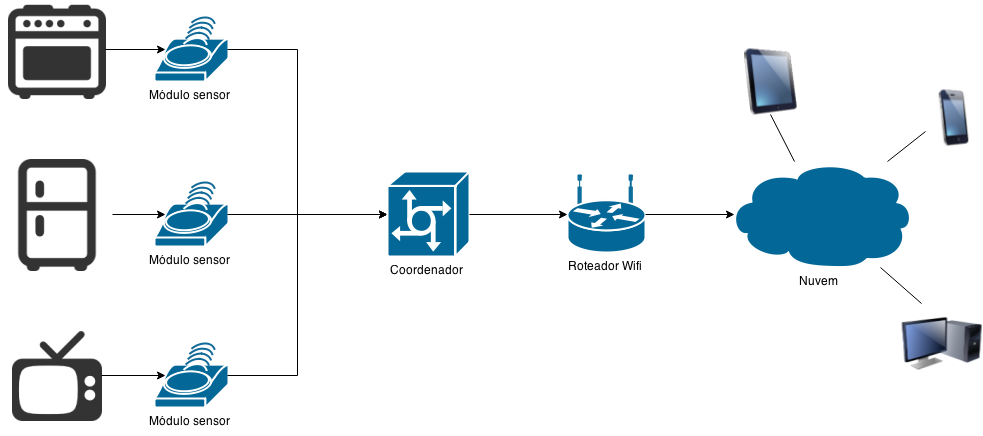
\includegraphics[width=1\textwidth]{figuras/esqueminha.png}
\caption{\label{fig:esqueminha} Esquema do Projeto}
\end{figure}

\begin{figure}
\centering
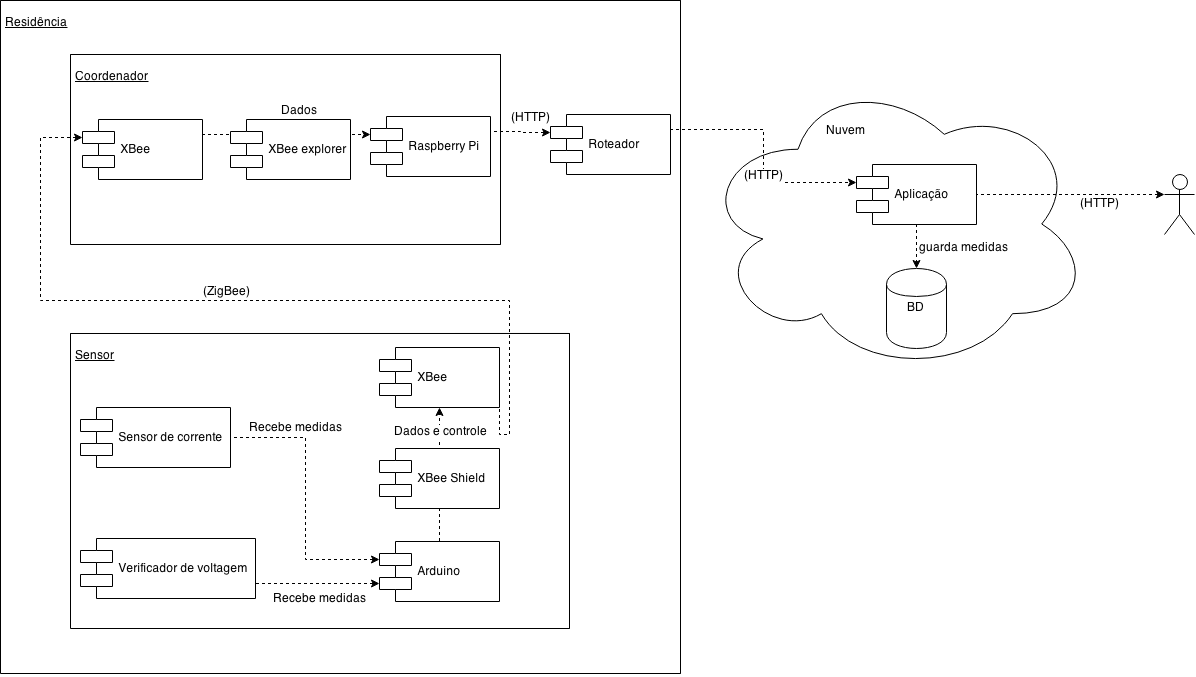
\includegraphics[width=1\textwidth]{figuras/diagrama_implantacao.png}
\caption{\label{fig:diagrama_implantacao} Diagrama de implantação}
\end{figure}

A parte de hardware está separado em dois módulos principais: o módulo de sensoriamento e um módulo coordenador e a parte de software se resume à parte da aplicação web na nuvem.

\section{Escopo}

Coletados os dados, resta mostrar informações úteis ao usuário. Com o consumo de corrente e a voltagem da tomada, é possível calcular a potência e alguns outros dados interessantes para o usuário. O aplicativo desenvolvido nesse trabalho será responsável por esse tratamento e a visualização dos dados coletados pelos sensores. As principais metas são as seguintes:

\begin{itemize}
	\item{informar ao usuário sobre o gasto de energia por equipamento em sua residência}
	\item{auxiliar o usuário a tomar decisões para diminuir o consumo de energia}
  \item{permitir o acesso às informações de consumo tanto localmente quanto remotamente}
\end{itemize}
%
\section{Funções do Sistema}

\begin{description}
	\item[Gerenciar contas:] O usuário poderá fazer cadastro/alteração de conta e autenticação.
	\item[Gerenciar equipamentos:] O usuário poderá fazer criação, edição e remoção de equipamentos, os quais serão monitorados pelo sistema
	\item[Gerenciar sensores:] Os módulos sensores são auto-detectados, e o usuário poderá editar ou removê-los
	\item[Gerenciar metas:] O usuário poderá criar, editar e remover metas mensais.
	\item[Gerenciar consumo:] O módulo coordenador enviará consumos para o sistema estes serão cadastrados. O usuário poderá visualizar os consumos através de gráficos. Além disso o usuário poderá importar ou exportar dados de consumo
	\item[Atualizar taxas da AES:] O usuário poderá atualizar as taxas de energia utilizadas para cálculo do custo do consumo
	\item[Configurar sistema:] O usuário poderá associar os sensores aos equipamentos e escolher um tipo de renda
\end{description}

\section{Requisitos não Funcionais}

\begin{itemize}
	\item{independência do usuário em relação ao técnico do sistema para instalar o sistema em sua residência}
	\item{sistema de fácil manuseio pelo usuário morador da residência}
	\item{os componentes físicos do sistema portáteis}
\end{itemize}

\section{Premissas}

Sendo esse um projeto que visa o sensoriamento e de um monitor para vizualisar os dados com o objetivo de dar uma visão geral ao usuário sobre gastos supérfulos e uma relação absoluta do consumo de cada equipamento, o sistema é influenciado por alguns fatores físicos e geopolíticos, o que leva à necessidade de usar algumas premissas que tiveram de ser feitas para ajustar o projeto ao tempo previsto e garantir o funcionamento correto do sistema:

\begin{enumerate}
\item{O usuário deve morar em São Paulo}
\item{Será considerado um fator de potência ideal unitário}
\end{enumerate}
\section{Hardware}
\label{Sec:hardware}
\subsection{Módulo sensor}

O módulo sensor vai ser responsável por medir e transmitir as informações necessárias para calcular o consumo de energia do equipamento acoplado.

Os componentes físicos do módulo sensor são:

\begin{itemize}
\item Circuito Verificador de tensão
\item Sensor de Corrente (Non-invasive AC Current Sensor)
\item Arduino Uno - R3
\item XBee Shield
\item XBee 2mW PCB Antenna - Series 2
\end{itemize}
%
\subsection{Coordenador}

O módulo coordenador vai ser responsável por fazer requisições para os módulos sensores, tratar os dados de consumo e enviar ao aplicativo na nuvem.

Os componentes do coordenador são:

\begin{itemize}
\item Kit Raspberry Pi2 + Fonte + Microsd 8gb + Wifi Usb
\item XBee Explorer Dongle
\item XBee 2mW PCB Antenna - Series 2
\end{itemize}
%
\subsection{Circuitos}
\subsubsection{Verificador de Tensão}

No circuito de cada módulo de sensor, são feitas detecções da tensão (127V ou 220V) para cálculos de potência.  O objetivo do circuito da figura \ref{fig:voltage-circuit} é indicar se a tensão na tomada é 220V ou 127V. A saída do circuito é usada como um valor analógico, que dependendo da tensão de entrada resultará em faixas diferentes para as diferentes tensões.

\begin{figure}[H]
\centering
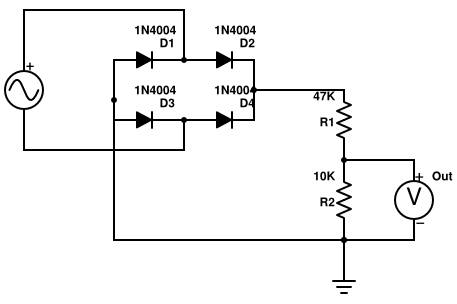
\includegraphics[width=9cm,keepaspectratio]{figuras/voltage-circuit.jpg}
\caption{\label{fig:voltage-circuit} Circuito verificador de tensão}
\end{figure}

\subsubsection{Medidor de Corrente}

Ainda no módulo sensor, é necessário obter as medidas do valor eficaz da corrente. O sensor não-invasivo produz uma tensão alternada na saída, e antes da coleta de dados pelo arduino é preciso obter um valor significativo, que não ultrapasse 2.5V. Para isso foi utilizado o circuito da figura \ref{fig:sensor-circuit}.

\begin{figure}[H]
\centering
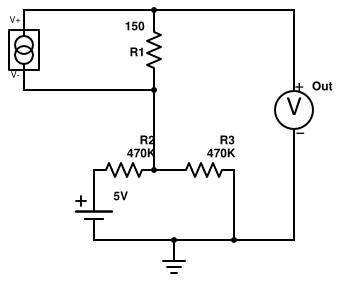
\includegraphics[width=9cm,keepaspectratio]{figuras/current-circuit.jpg}
\caption{\label{fig:sensor-circuit} Circuito medidor de corrente}
\end{figure}
%
\subsection{Peças}
\subsubsection{Sensor de Corrente Não-invasivo AC}
\begin{figure}[H]
\begin{center}
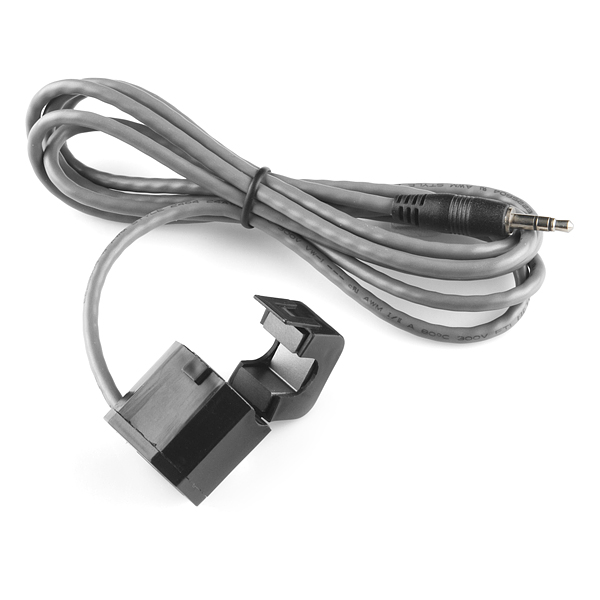
\includegraphics[width=5cm,height=5cm,keepaspectratio]{figuras/sensor.jpg}
\caption{\label{fig:sensor} Non-invasive AC current sensor}
\end{center}
\end{figure}

Esse sensor de corrente consegue medir a corrente que passa por um fio de modo não-invasivo. O sensor funciona como um transformador respondendo a um campo magnético formado em volta do fio condutor. Este, em particular, suporta até 30A de entrada, e necessita de um resistor de saída para obter a medida desejada em tensão.

\begin{itemize}
\item{Corrente suportada: 30A}
\item{Temperatura de operação: -40$^{\circ}$C até 65 $^{\circ}$C}
\item{Precisão de 2\%}
\end{itemize}
%
\subsubsection{Raspberry Pi 2 modelo B}
\begin{figure}[H]
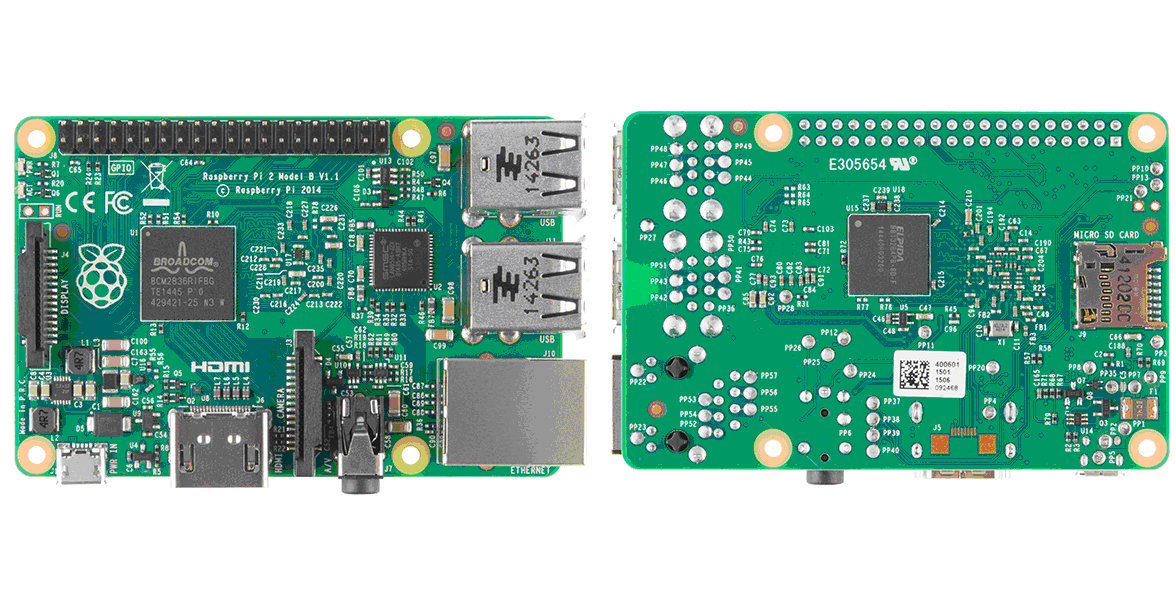
\includegraphics[width=1\textwidth]{figuras/raspberry_pi.png}
\caption{\label{fig:raspberry pi} Raspberry pi 2 modelo B}
\end{figure}

A Raspberry Pi 2 Modelo B (figura \ref{fig:raspberry pi}) é o computador utilizado no sistema para receber os dados enviados pelos módulos sensores, tratá-los e enviar para o aplicativo. Foi escolhido o Raspberry Pi 2 - Model B por ser mais veloz, por possuir mais entradas USB e ser de alta disponibilidade no mercado, por um preço razoável. O kit inclui a fonte, um cartão microSD de 8GB e um adaptador Wifi USB.

\begin{itemize}
\item{A 900MHz quad-core ARM Cortex-A7 CPU}
\item{1GB RAM}
\item{40 pinos GPIO}
\item{saída Full HDMI}
\item{porta Ethernet}
\item{entrada para cartão Micro SD}
\item{4 entradas USB}
\end{itemize}
%
\subsubsection{Arduino UNO}
\begin{figure}[H]
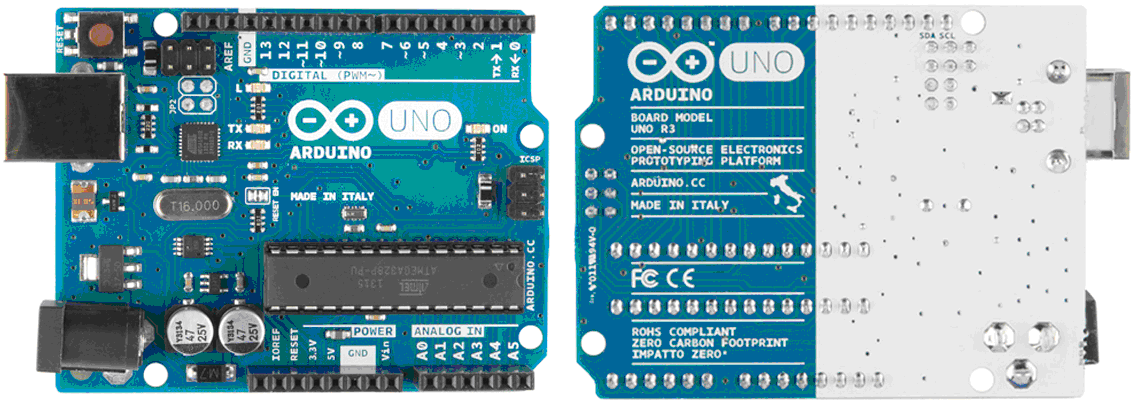
\includegraphics[width=1\textwidth]{figuras/arduino_uno.png}
\caption{\label{fig:arduino uno} Arduino UNO R3}
\end{figure}

Arduino é uma placa programável open-source . No projeto em questão esse componente receberá os dados do sensor, fará um tratamento e terá o envio programado desses para o coordenador. Pelo Arduino ser programável e possuir uma interface muito amigável, simplifica essa ponte entre a coleta de dados e a transmissão. E sua alta disponibilidade no mercado , assim como o raspberry, facilita sua obtenção.

\begin{itemize}
\item{microcontrolador ATmega328}
\item{tensão de entrada - 7-12V}
\item{14 Pinos Digital I/O (6 PWM de saída)}
\item{6 Inputs Analógicos}
\item{32k de memória Flash}
\item{16Mhz de Relógio}
\end{itemize}
%
\subsubsection{XBee}
\begin{figure}[H]
\begin{center}
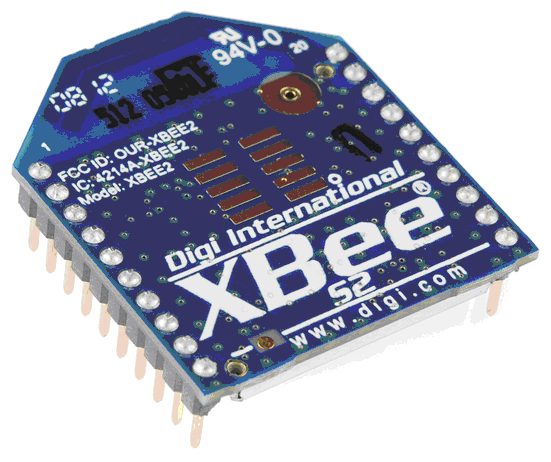
\includegraphics[width=5cm,height=5cm,keepaspectratio]{figuras/xbee_serie2.png}
\caption{\label{fig:xbee} XBee Serie 2}
\end{center}
\end{figure}

É um módulo que permite uma comunicação simples e confiável entre microcontroladores, computadores, sistemas através de uma porta serial com um consumo menor de energia. Pode ser utilizado em redes ponto-a-ponto e multi-ponto. Foram escolhidos módulos da série 2 por serem configuráveis.
Algumas outras especificações são:

\begin{itemize}
\item{entradas de 3.3V @ 40mA}
\item{transmissão de dados máxima de 250kbps}
\item{potência de saída: 2mW (+3dBm)}
\item{alcance máximo de 120m}
\item{08 pinos digitais entrada/saída}
\item{encriptação 128-bit}
\item{configuração local ou remota}
\item{conector de antena RPSMA}
\end{itemize}
%
\subsubsection{XBee Explorer Dongle}
\begin{figure}[H]
\begin{center}
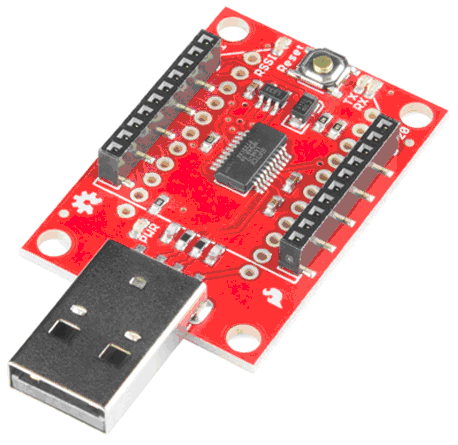
\includegraphics[width=5cm,height=5cm,keepaspectratio]{figuras/xbee_explorer_dongle.png}
\caption{\label{fig:xbee explorer dongle} XBee Explorer Dongle}
\end{center}
\end{figure}

É um módulo com porta USB que faz a conexão do módulo XBee a um computador. Isso é necessário para ter acesso aos pinos de comunicação serial e de programação. Ele possui um conversor serial, que traduz os dados entre o computador e o XBee. Possui um botão de reset e um regulador de tensão para suprir a tensão necessária para XBee. Além disso possui 4 leds para debug: RX, TX, RSSI e indicador de energia. No projeto, este módulo é utilizado para fazer as configurações iniciais de todos os XBees e para conectar o XBee coordenador ao Raspberry Pi. Apesar de não ser um dispositivo essencial, este facilita muito nas tarefas citadas,  principalmente por lidar com a alimentação de 3,3V do XBee.

\subsubsection{XBee Shield}
\begin{figure}[H]
\begin{center}
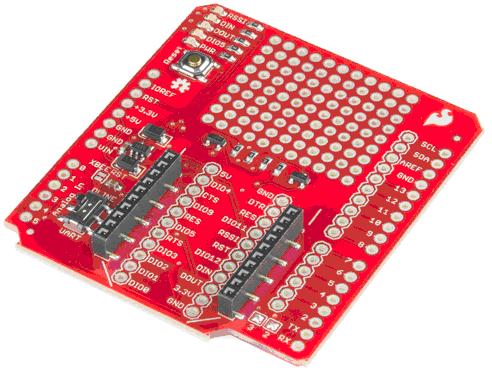
\includegraphics[width=5cm,height=5cm,keepaspectratio]{figuras/xbee_shield.png}
\caption{\label{fig:xbee shield} XBee shield do arduino UNO}
\end{center}
\end{figure}

É um módulo que faz a conexão entre um módulo XBee e um Arduino. Ele possui opções para escolher se a conexão vai ser nos pinos UART ou qualquer outros pinos digitais do Arduino. A alimentação de 5V vinda do Arduino é regulada para 3.3V VDC antes de chegar no módulo XBee. O XBee Shield inclui LEDs para indicar a utilização dos pinos DIN, DOUT, RSSI e DIO5 do XBee. É usado um módulo XBee Shield para cada par XBee + Arduino.

\subsubsection{Arduino Stackable Header Kit - R3}
\begin{figure}[H]
\begin{center}
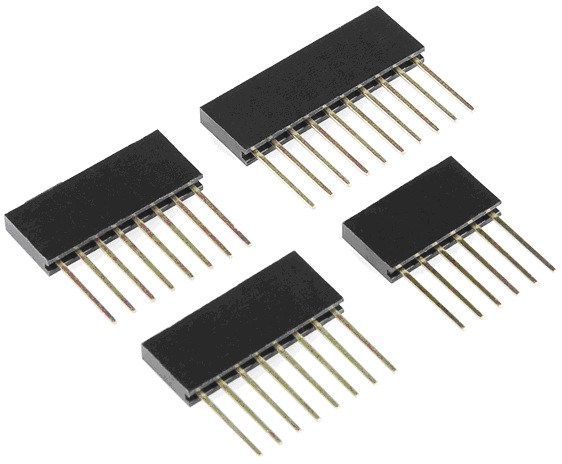
\includegraphics[width=5cm,height=5cm,keepaspectratio]{figuras/headers.png}
\caption{\label{fig:xbee shield headers} Headers usados no XBee shield}
\end{center}
\end{figure}

São conectores usados para encaixar o módulo XBee Shield no Arduino Uno R3. Estão inclusos 4 headers, 2 x 8 pinos, 1 x 10 pinos e 1 x 6 pinos, suficientes para 1 módulo XBee Shield. Como há 2 sensores no projeto, serão usados 2 kits, com um adicional de reserva.



\section{Software}
\label{Sec:software}

\subsection{Classes e atributos}

A seguir estão descritas as classes do sistema e seus respectivos atributos. As classes implementadas estão representadas pelo diagrama de classes (figura \ref{fig:diagrama-classes}).

\begin{figure}[H]
\begin{center}
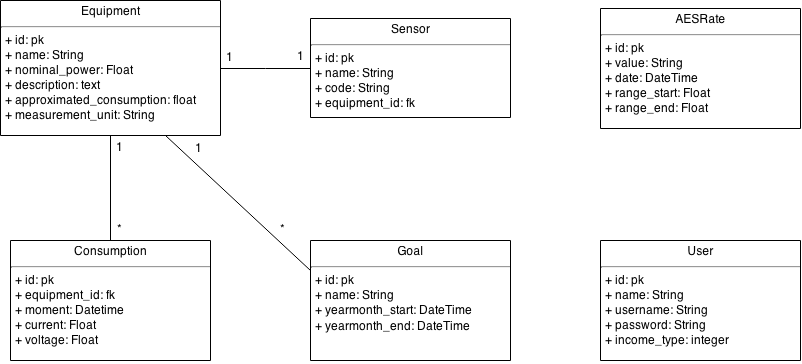
\includegraphics[width=10cm,height=10cm,keepaspectratio]{figuras/diagrama_classes.png}
\caption{\label{fig:diagrama-classes} Diagrama de Classes}
\end{center}
\end{figure}

\subsubsection{Equipment}
\begin{description}
	\item[Classe:] Equipment
	\item[Descrição:] um equipamento monitorado
	\item[Atributos:]
\end{description} 
\begin{enumerate}
  \item id (integer): Identificador do equipamento
  \item name (String): Nome do equipamento
  \item description (Text): descrição do equipamento 
  \item nominal\_power (float): potência do equipamento descrita no manual do equipamento 
  \item measurement\_unit (String): unidade do valor dado em nominal\_power
  \item approximated\_consumption (float): consumo aproximado do equipamento dado pelo fabricante 
\end{enumerate}
%
\subsubsection{Sensor}
\begin{description}
	\item[Classe:] Sensor
	\item[Descrição:] um sensor do sistema
	\item[Atributos:]
\end{description} 
\begin{enumerate}
	\item id (integer): identificador do sensor dentro do software.
	\item name (String): nome dado pelo usuário para o sensor
	\item code (String): identificador do sensor entre outros sensores. Informação configurada no próprio módulo do sensor.
	\item equipment\_id (integer): equipamento a qual está associado
\end{enumerate}
%
\subsubsection{Consumption}
\begin{description}
	\item[Classe:] Consumption
	\item[Descrição:] Representa uma medida feita de um equipamento em um dado instante
	\item[Atributos:]
\end{description} 
\begin{enumerate}
	\item id (integer): identificador do consumo
	\item moment (DateTime): a data e a hora de quando foi feita a medida
	\item current (float): corrente no momento da medida em amperes
	\item voltage (float): voltagem do tomada do equipamento. 220V ou 110V
\end{enumerate}
%
\subsubsection{User}
\begin{description}
	\item[Classe:] User
	\item[Descrição:] Representa um usuário do sistema
	\item[Atributos:]
\end{description} 
\begin{enumerate}
	\item id (integer): identificador do usuário
	\item name (String):  Nome do usuário
	\item username (String): Nome de usuário usado para efetuar o login
	\item password (String com Criptografia): Senha do usuário usada para efetuar o login
    \item income\_type (String): O tipo de renda do usuário, Residencial ou Residencial de baixa renda, definida pela AES eletropaulo.
\end{enumerate}
%
\subsubsection{Goal}
\begin{description}
	\item[Classe:] Goal
	\item[Descrição:] Representa uma meta de consumo por mês
	\item[Atributos:]
\end{description} 
\begin{enumerate}
	\item id (integer): identificador da meta
	\item name (String):  Nome da meta
	\item value\_in\_percent (float): Consumo pretendido em percentagem (em relação ao mês anterior)
	\item yearmonth\_start (DateTime): Mês/Ano de início do período da meta
    \item yearmonth\_end (DateTime): Mês/Ano de fim do período da meta
\end{enumerate}
%
\subsubsection{AESRate}
\begin{description}
	\item[Classe:] AESRate
	\item[Descrição:] Representa a taxa de conversão da AES eletropaulo de kilowatts hora para reais. Esses valores obtidos através da página de tarifas do site da AES Eletropaulo \cite{aes_site}
	\item[Atributos:]
\end{description} 
\begin{enumerate}
	\item id (integer): identificador da taxa de conversão
	\item value (float): O valor da taxa de conversão no instante
	\item date (DateTime): O instante que a taxa de conversão foi buscada
	\item range\_start (float): O início da faixa que define a taxa de conversão
    \item range\_end (float): O início da faixa que define a taxa de conversão
\end{enumerate}

No sistema é possível cadastrar apenas uma entidade principal os equipamentos eletrônicos monitorados, sendo prevista a possibilidade de que um sensor possa mudar de um equipamento para outro, sendo que tal mudança deve ser cadastrada no sistema pelo  usuário na tela de configurações, como mostrado na tela de configurações no diagrama de navegação (figura \ref{fig:diagrama-navegacao}).  Essa possibilidade de mudança da configuração dos sensores explica a relação do equipamento e as medidas de consumo: caso o usuário troque o sensor de equipamento ainda será possível visualizar dados anteriores de outros equipamentos já monitorados.

Os sensores devem ser criados automaticamente pelo sistema uma vez que eles sejam colocados no sistema. Eles enviam um sinal inicial que informa seu identificador para que o sistema o cadastre. O usuário poderá, então, colocar um nome que preferir nesse sensor. Porém, como não há qualquer informação que o sistema pode indicar ao sistema em qual aparelho ou em que tipo de aparelho o sensor foi instalado, tal associação deve ser feita manualmente antes que os dados comecem a ser coletados.

Adquiridas as medidas, é possível vizualizar esses dados em uma tabela de consumo na tela de consumo. Nessa tela, é possível construir o gráfico do consumo em função de vários períodos de tempo, no caso, o consumo por dia e por mês, assim como metas de consumo de energia dos equipamentos selecionados e previsões de consumo que serão calculadas a partir do consumo nominal dos equipamentos.

\begin{figure}[H]
\begin{center}
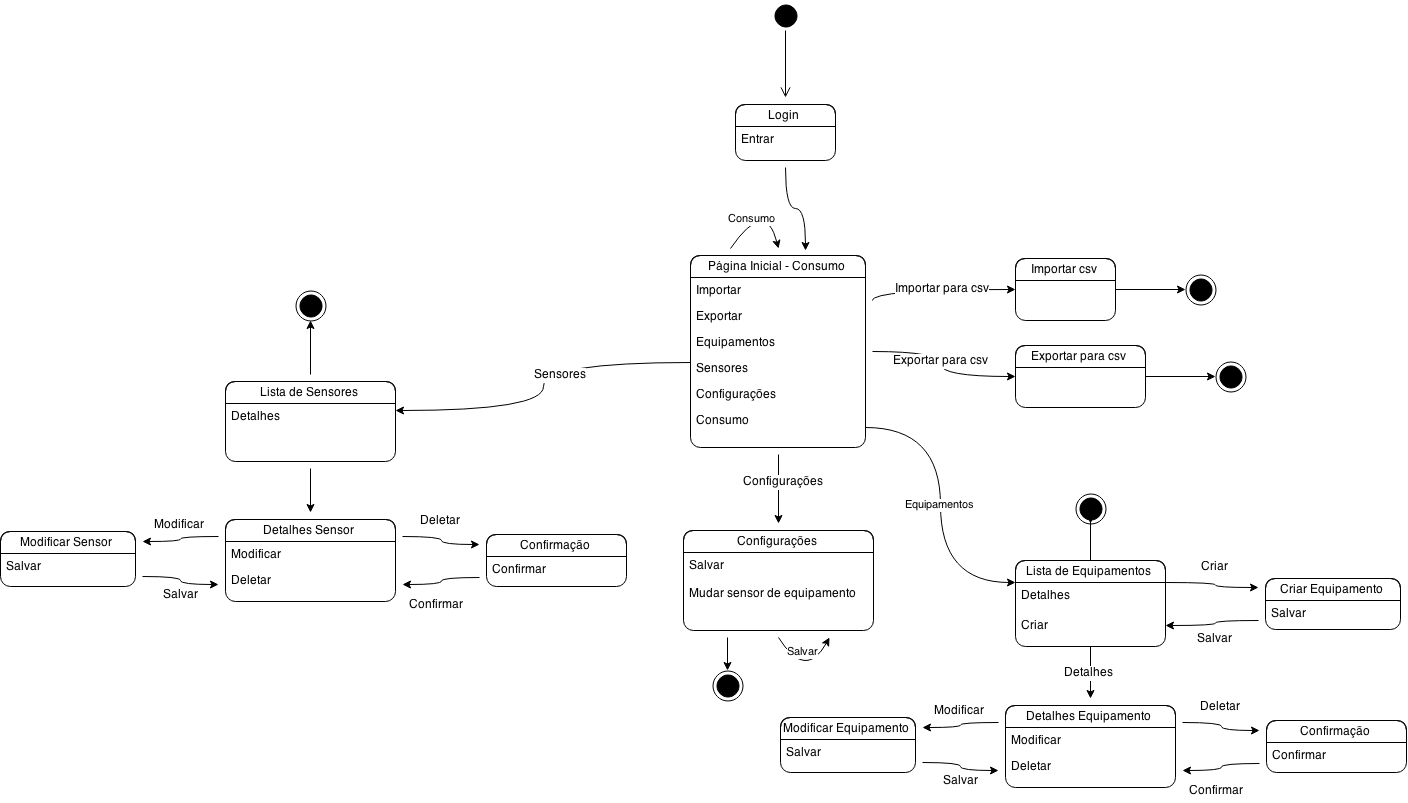
\includegraphics[width=10cm,height=10cm,keepaspectratio]{figuras/diagrama_navegacao.png}
\caption{\label{fig:diagrama-navegacao} Diagrama de Navegação}
\end{center}
\end{figure}
%
\subsection{Atores}
\begin{description}
	\item[usuário:] Como o sistema vai ser utilizado apenas pelo(s) responsável(is) pela residência, há apenas um tipo de usuário, que é o usuário comum
    \item[módulo coordenador:] É o componente de hardware que enviará informações de consumo para o sistema
\end{description}
\subsection{Casos de uso}

Os casos de uso do sistema estão listados na tabela \ref{tab:casos_de_uso}.

\begin{table}
\centering
{\renewcommand{\arraystretch}{1.5}
\renewcommand{\tabcolsep}{0.2cm}
\begin{tabular}{|c|c|}
\hline
\textbf{Funções} & \textbf{Casos de uso} \\
\hline
\multirow{4}{*}{Gerenciar conta} & Fazer cadastro\\
& Fazer login\\
& Fazer logout\\
& Recuperar senha\\
\hline
\multirow{3}{*}{Gerenciar equipamentos} & Criar equipamento\\
& Editar equipamento\\
& Remover equipamento\\
\hline
\multirow{3}{*}{Gerenciar sensores} & Detectar sensores\\
& Editar sensor\\
& Remover sensor\\
\hline
\multirow{3}{*}{Gerenciar metas} & Criar meta\\
& Editar meta\\
& Remover meta\\
\hline
\multirow{4}{*}{Gerenciar consumo} & Criar consumo\\
& Visualizar consumo\\
& Importar consumo\\
& Exportar consumo\\
\hline
Atualizar taxas da AES & Atualizar taxas da AES\\
\hline
Configurar sistema & Configurar sistema\\
\hline
\end{tabular}}
\caption{\label{tab:casos_de_uso} Casos de Uso.}
\end{table}
%
\subsection{Descrição dos casos de uso}

A seguir são descritos os casos de uso do sistema. 

% ************************************************
% 1 - GERENCIAR CONTA
% ************************************************
\subsubsection{Caso de Uso 1: Gerenciar conta}
\subsubsection{Caso de Uso 1.1: Fazer cadastro}
\begin{description}
	\item[Descrição:] inserção de um novo usuário comum no sistema
	\item[Evento iniciador:] solicitação de cadastro
	\item[Atores:] usuário
	\item[Pré-condição:] sistema exibindo tela de solicitação de cadastro
	\item[Sequência de eventos:] \hfill
		\begin{enumerate}
			\item{Usuário solicita cadastro}
			\item{Sistema exibe o formulário de cadastro}
			\item{Usuário insere os seus dados}
			\item{Sistema insere o novo usuário e exibe o resultado}
		\end{enumerate}
	\item[Pós-condição:] novo usuário cadastrado, usuário é logado automaticamente e é exibida a tela inicial
	\item[Extensões:] \hfill
		\begin{enumerate}
			\item{\textbf{Usuário a ser cadastrado já existe:} sistema apresenta uma mensagem ao usuário (passo 4)}
			\item{\textbf{Dados do usuário não consistentes:} sistema apresenta mensagem de erro ao usuário (passo 4)}
		\end{enumerate}
	\item[Inclusões:] \hfill
		\begin{enumerate}
			\item{Buscar usuário (passo 4)}
		\end{enumerate}
\end{description}
%
\subsubsection{Caso de Uso 1.2: Fazer login}
\begin{description}
	\item[Descrição:] criar uma sessão do usuário no sistema
	\item[Evento iniciador:] solicitação de login
	\item[Atores:] usuário
	\item[Pré-condição:] usuário cadastrado e não há usuário logado
	\item[Sequência de eventos:] \hfill
		\begin{enumerate}
			\item{usuário solicita login}
			\item{sistema exibe formulário para login}
			\item{usuário insere os dados de login}
			\item{sistema cria uma sessão para o usuário e redireciona para a página inicial}
		\end{enumerate}
	\item[Pós-condição:] sessão criada e sistema exibe a tela inicial
	\item[Extensões:] \hfill
		\begin{enumerate}
			\item{\textbf{Usuário não encontrado:} sistema apresenta uma mensagem de erro ao usuário (passo 4)}
			\item{\textbf{Dados não consistentes:} sistema apresenta uma mensagem de erro ao usuário (passo 4)}
		\end{enumerate}
	\item[Inclusões:] \hfill
		\begin{enumerate}
			\item{Buscar usuário (passo 4)}
		\end{enumerate}
\end{description}
%
\subsubsection{Caso de Uso 1.3: Fazer logout}
\begin{description}
	\item[Descrição:] encerrar a sessão do usuário atual no sistema
	\item[Evento iniciador:] solicitação de logout
	\item[Atores:] usuário
	\item[Pré-condição:] usuário logado
	\item[Sequência de eventos:] \hfill
		\begin{enumerate}
			\item{usuário solicita logout}
			\item{sistema encerra a sessão atual, e redireciona para a página de login}
		\end{enumerate}
	\item[Pós-condição:] sessão encerrada e sistema exibe tela de login
\end{description}
%
\subsubsection{Caso de Uso 1.4: Recuperar senha}
\begin{description}
	\item[Descrição:] recuperar a senha do usuário
	\item[Evento iniciador:] solicitação de recuperação de senha
	\item[Atores:] usuário
	\item[Pré-condição:] usuário cadastrado, não há usuário logado e sistema exibindo tela de login
	\item[Sequência de eventos:] \hfill
		\begin{enumerate}
			\item{usuário solicita recuperação de senha}
			\item{sistema exibe formulário para recuperação de senha}
			\item{usuário insere o e-mail}
			\item{sistema envia e-mail para recuperar a senha e exibe mensagem}
			\item{usuário clica no link para recuperar senha no e-mail}
			\item{sistema exibe o formulário para recuperar a senha}
			\item{usuário insere os dados pedidos}
			\item{sistema atualiza a senha do usuário, autentica o usuário e redireciona para a tela inicial}
		\end{enumerate}
	\item[Pós-condição:] senha do usuário atualizada, usuário autenticado e sistema mostra a tela inicial
	\item[Extensões:] \hfill
		\begin{enumerate}
			\item{\textbf{Dados não consistentes:} sistema apresenta uma mensagem de erro ao usuário (passo 4, 8)}
			\item{\textbf{Senha antiga incorreta:} sistema apresenta uma mensagem de erro ao usuário (passo 8)}
		\end{enumerate}
	\item[Inclusões:] \hfill
		\begin{enumerate}
			\item{Buscar usuário (passo 8)}
		\end{enumerate}
\end{description}
% ************************************************
% 2 - GERENCIAR EQUIPAMENTO
% ************************************************
\subsubsection{Caso de Uso 2: Gerenciar equipamentos}
\subsubsection{Caso de Uso 2.1: Criar equipamento}
\begin{description}
	\item[Descrição:] criar um novo equipamento
	\item[Evento iniciador:] solicitação de criação de equipamento
	\item[Atores:] usuário
	\item[Pré-condição:] usuário logado e sistema exibindo listagem de equipamentos
	\item[Sequência de eventos:] \hfill
		\begin{enumerate}
			\item{usuário solicita criação de equipamento}
			\item{sistema exibe formulário para criação}
			\item{usuário insere os dados para criação}
			\item{sistema cria um equipamento e redireciona para a listagem de equipamentos}
		\end{enumerate}
	\item[Pós-condição:] equipamento criado e sistema exibe listagem de equipamentos
	\item[Extensões:] \hfill
		\begin{enumerate}
			\item{\textbf{Dados não consistentes:} sistema apresenta uma mensagem de erro ao usuário (passo 4)}
			\item{\textbf{Equipamento já existe:} sistema apresenta uma mensagem de erro ao usuário (passo 4)}
		\end{enumerate}
	\item[Inclusões:] \hfill
		\begin{enumerate}
			\item{Buscar equipamento (passo 4)}
		\end{enumerate}
\end{description}
%
\subsubsection{Caso de Uso 2.2: Editar equipamento}
\begin{description}
	\item[Descrição:] editar um equipamento
	\item[Evento iniciador:] solicitação de edição de equipamento
	\item[Atores:] usuário
	\item[Pré-condição:] usuário logado, existem equipamentos e sistema exibindo listagem de equipamentos
	\item[Sequência de eventos:] \hfill
		\begin{enumerate}
			\item{usuário seleciona o equipamento desejado para edição}
			\item{sistema exibe formulário para edição}
			\item{usuário altera os dados desejados}
			\item{sistema atualiza o equipamento e redireciona para a listagem de equipamentos}
		\end{enumerate}
	\item[Pós-condição:] equipamento atualizado e sistema exibe listagem de equipamentos
	\item[Extensões:] \hfill
		\begin{enumerate}
			\item{\textbf{Dados não consistentes:} sistema apresenta uma mensagem de erro ao usuário (passo 4)}
		\end{enumerate}
	\item[Inclusões:] \hfill
		\begin{enumerate}
			\item{Buscar equipamento (passo 2, 4)}
		\end{enumerate}
\end{description}
%
\subsubsection{Caso de Uso 2.3: Remover equipamento}
\begin{description}
	\item[Descrição:] remover um equipamento
	\item[Evento iniciador:] solicitação de remoção de equipamento
	\item[Atores:] usuário
	\item[Pré-condição:] usuário logado, existem equipamentos e sistema exibindo listagem de equipamentos
	\item[Sequência de eventos:] \hfill
		\begin{enumerate}
			\item{usuário seleciona o equipamento desejado para remoção}
			\item{sistema pede confirmação para remoção}
			\item{usuário confirma}
			\item{sistema remove o equipamento e redireciona para a listagem de equipamentos}
		\end{enumerate}
	\item[Pós-condição:] equipamento removido e sistema exibe listagem de equipamentos
	\item[Extensões:] \hfill
		\begin{enumerate}
			\item{\textbf{Usuário não confirma:} sistema não remove e volta para a tela de listagem (passo 4)}
		\end{enumerate}
	\item[Inclusões:] \hfill
		\begin{enumerate}
			\item{Buscar equipamento (passo 2, 4)}
		\end{enumerate}
\end{description}
% ************************************************
% 3 - GERENCIAR SENSORES
% ************************************************
\subsubsection{Caso de Uso 3: Gerenciar sensores}
\subsubsection{Caso de Uso 3.1: Detectar sensor}
\begin{description}
	\item[Descrição:] detectar um sensor
	\item[Evento iniciador:] solicitação de detecção de sensores
	\item[Atores:] usuário
	\item[Pré-condição:] usuário logado e sistema exibindo listagem de sensores
	\item[Sequência de eventos:] \hfill
		\begin{enumerate}
			\item{usuário solicita detecção de sensor}
			\item{sistema detecta e cria um sensor no sistema com status ativo e atualiza a lista de sensores}
		\end{enumerate}
	\item[Pós-condição:] sensor criado e sistema exibe listagem de sensores
	\item[Extensões:] \hfill
		\begin{enumerate}
			\item{\textbf{Sensor já existe no sistema:} sistema atualiza o status do sensor para ativo (passo 2)}
		\end{enumerate}
	\item[Inclusões:] \hfill
		\begin{enumerate}
			\item{Buscar sensor (passo 2)}
		\end{enumerate}
\end{description}
%
\subsubsection{Caso de Uso 3.2: Editar sensor}
\begin{description}
	\item[Descrição:] editar um sensor
	\item[Evento iniciador:] solicitação de edição de sensor
	\item[Atores:] usuário
	\item[Pré-condição:] usuário logado, existem sensores e sistema exibindo listagem de sensores
	\item[Sequência de eventos:] \hfill
		\begin{enumerate}
			\item{usuário seleciona o sensor desejado para edição}
			\item{sistema exibe formulário para edição}
			\item{usuário altera os dados desejados}
			\item{sistema atualiza o sensor e redireciona para a listagem de sensores}
		\end{enumerate}
	\item[Pós-condição:] sensor atualizado e sistema exibe listagem de sensores
	\item[Extensões:] \hfill
		\begin{enumerate}
			\item{\textbf{Dados não consistentes:} sistema apresenta uma mensagem de erro ao usuário (passo 4)}
		\end{enumerate}
	\item[Inclusões:] \hfill
		\begin{enumerate}
			\item{Buscar sensor (passo 2, 4)}
		\end{enumerate}
\end{description}
%
\subsubsection{Caso de Uso 3.3: Remover sensor}
\begin{description}
	\item[Descrição:] remover um sensor
	\item[Evento iniciador:] solicitação de remoção de sensor
	\item[Atores:] usuário
	\item[Pré-condição:] usuário logado, existem sensores e sistema exibindo listagem de sensores
	\item[Sequência de eventos:] \hfill
		\begin{enumerate}
			\item{usuário seleciona o sensor desejado para remoção}
			\item{sistema pede confirmação para remoção}
			\item{usuário confirma}
			\item{sistema remove o sensor e redireciona para a listagem de sensores}
		\end{enumerate}
	\item[Pós-condição:] sensor removido e sistema exibe listagem de sensores
	\item[Extensões:] \hfill
		\begin{enumerate}
			\item{\textbf{Usuário não confirma:} sistema não remove e volta para a tela de listagem (passo 4)}
		\end{enumerate}
	\item[Inclusões:] \hfill
		\begin{enumerate}
			\item{Buscar sensor (passo 2, 4)}
		\end{enumerate}
\end{description}
% ************************************************
% 4 - GERENCIAR META
% ************************************************
\subsubsection{Caso de Uso 4: Gerenciar metas}
\subsubsection{Caso de Uso 4.1: Criar meta}
\begin{description}
	\item[Descrição:] criar uma nova meta
	\item[Evento iniciador:] solicitação de criação de meta
	\item[Atores:] usuário
	\item[Pré-condição:] usuário logado e sistema exibindo listagem de metas
	\item[Sequência de eventos:] \hfill
		\begin{enumerate}
			\item{usuário solicita criação de meta}
			\item{sistema exibe formulário para criação}
			\item{usuário insere os dados para criação}
			\item{sistema cria uma meta e redireciona para a listagem de metas}
		\end{enumerate}
	\item[Pós-condição:] meta criada e sistema exibe listagem de metas
	\item[Extensões:] \hfill
		\begin{enumerate}
			\item{\textbf{Dados não consistentes:} sistema apresenta uma mensagem de erro ao usuário (passo 4)}
			\item{\textbf{Meta já existe:} sistema apresenta uma mensagem de erro ao usuário (passo 4)}
		\end{enumerate}
	\item[Inclusões:] \hfill
		\begin{enumerate}
			\item{Buscar meta (passo 4)}
		\end{enumerate}
\end{description}
%
\subsubsection{Caso de Uso 4.2: Editar meta}
\begin{description}
	\item[Descrição:] editar uma meta
	\item[Evento iniciador:] solicitação de edição de meta
	\item[Atores:] usuário
	\item[Pré-condição:] usuário logado, existem metas e sistema exibindo listagem de metas
	\item[Sequência de eventos:] \hfill
		\begin{enumerate}
			\item{usuário seleciona a meta desejado para edição}
			\item{sistema exibe formulário para edição}
			\item{usuário altera os dados desejados}
			\item{sistema atualiza a meta e redireciona para a listagem de metas}
		\end{enumerate}
	\item[Pós-condição:] meta atualizada e sistema exibe listagem de metas
	\item[Extensões:] \hfill
		\begin{enumerate}
			\item{\textbf{Dados não consistentes:} sistema apresenta uma mensagem de erro ao usuário (passo 4)}
		\end{enumerate}
	\item[Inclusões:] \hfill
		\begin{enumerate}
			\item{Buscar meta (passo 2, 4)}
		\end{enumerate}
\end{description}
%
\subsubsection{Caso de Uso 4.3: Remover meta}
\begin{description}
	\item[Descrição:] remover uma meta
	\item[Evento iniciador:] solicitação de remoção de meta
	\item[Atores:] usuário
	\item[Pré-condição:] usuário logado, existem metas e sistema exibindo listagem de metas
	\item[Sequência de eventos:] \hfill
		\begin{enumerate}
			\item{usuário seleciona a meta desejado para remoção}
			\item{sistema pede confirmação para remoção}
			\item{usuário confirma}
			\item{sistema remove a meta e redireciona para a listagem de metas}
		\end{enumerate}
	\item[Pós-condição:] meta removida e sistema exibe listagem de metas
	\item[Extensões:] \hfill
		\begin{enumerate}
			\item{\textbf{Usuário não confirma:} sistema não remove e volta para a tela de listagem (passo 4)}
		\end{enumerate}
	\item[Inclusões:] \hfill
		\begin{enumerate}
			\item{Buscar meta (passo 2, 4)}
		\end{enumerate}
\end{description}
% ************************************************
% 5 - GERENCIAR CONSUMO
% ************************************************
\subsubsection{Caso de Uso 5: Gerenciar consumos}
\subsubsection{Caso de Uso 5.1: Criar consumo}
\begin{description}
	\item[Descrição:] inserir consumos no sistema
	\item[Evento iniciador:] solicitação para criação de consumo
	\item[Atores:] módulo coordenador
	\item[Pré-condição:] módulo coordenador ligado e sistema online
	\item[Sequência de eventos:] \hfill
		\begin{enumerate}
			\item{módulo coordenador solicita criação de consumo}
			\item{sistema cria o consumo}
		\end{enumerate}
	\item[Pós-condição:] consumo criado
	\item[Extensões:] \hfill
		\begin{enumerate}
			\item{\textbf{Perda de conexão:} consumo não é criado (passo 2)}
		\end{enumerate}
\end{description}
%
\subsubsection{Caso de Uso 5.2: Visualizar consumo}
\begin{description}
	\item[Descrição:] visualizar os consumos na forma de gráficos
	\item[Evento iniciador:] solicitação de geração de gráfico
	\item[Atores:] usuário
	\item[Pré-condição:] usuário logado, existem consumos e sistema exibindo tela de consumo
	\item[Sequência de eventos:] \hfill
		\begin{enumerate}
			\item{usuário configura os parâmetros e solicita geração do gráfico}
			\item{sistema exibe o gráfico de consumo}
		\end{enumerate}
	\item[Pós-condição:] sistema exibe gráfico de consumo
	\item[Extensões:] \hfill
		\begin{enumerate}
			\item{\textbf{Dados não consistentes:} sistema apresenta uma mensagem de erro ao usuário (passo 2)}
		\end{enumerate}
	\item[Inclusões:] \hfill
		\begin{enumerate}
			\item{Buscar consumos (passo 2)}
		\end{enumerate}
\end{description}
%
\subsubsection{Caso de Uso 5.3: Importar consumos}
\begin{description}
	\item[Descrição:] importar consumos por csv
	\item[Evento iniciador:] solicitação de importação de consumos
	\item[Atores:] usuário
	\item[Pré-condição:] usuário logado, sistema exibindo tela de consumo
	\item[Sequência de eventos:] \hfill
		\begin{enumerate}
			\item{usuário insere o arquivo csv e solicita importação de consumos}
			\item{sistema lê o csv, cria os consumos e exibe tela de consumo}
		\end{enumerate}
	\item[Pós-condição:] novos consumos criados e sistema exibe tela de consumo
	\item[Extensões:] \hfill
		\begin{enumerate}
			\item{\textbf{Dados não consistentes:} sistema apresenta uma mensagem de erro ao usuário (passo 2)}
		\end{enumerate}
\end{description}
%
\subsubsection{Caso de Uso 5.4: Exportar consumos}
\begin{description}
	\item[Descrição:] exportar consumos por csv
	\item[Evento iniciador:] solicitação de exportação de consumos
	\item[Atores:] usuário
	\item[Pré-condição:] usuário logado, existem consumos e sistema exibindo tela de consumo
	\item[Sequência de eventos:] \hfill
		\begin{enumerate}
			\item{usuário seleciona o período desejado do consumo para exportação}
			\item{sistema disponibiliza o download do csv}
		\end{enumerate}
	\item[Pós-condição:] sistema exibe arquivo de csv
	\item[Inclusões:] \hfill
		\begin{enumerate}
			\item{Buscar consumo (passo 2)}
		\end{enumerate}
\end{description}
% ************************************************
% 6 - ATUALIZAR TAXAS DA AES
% ************************************************
\subsubsection{Caso de Uso 6: Atualizar taxas da AES}
\begin{description}
	\item[Descrição:] atualizar dados de custo da AES Eletropaulo no sistema
	\item[Evento iniciador:] solicitação de atualização das taxas
	\item[Atores:] usuário
	\item[Pré-condição:] usuário logado e sistema exibindo tela de listagem de taxas
	\item[Sequência de eventos:] \hfill
		\begin{enumerate}
			\item{usuário solicita atualização de taxas}
			\item{sistema busca dados do site da AES Eletropaulo e cria taxas no sistema}
		\end{enumerate}
	\item[Pós-condição:] taxas criadas e sistema exibe listagem de taxas
	\item[Extensões:] \hfill
		\begin{enumerate}
			\item{\textbf{Taxa já existe no sistema:} sistema atualiza a taxa correspondente (passo 2)}
		\end{enumerate}
	\item[Inclusões:] \hfill
		\begin{enumerate}
			\item{Buscar taxa (passo 2)}
		\end{enumerate}
\end{description}
% ************************************************
% 7 - CONFIGURAR SISTEMA
% ************************************************
\subsubsection{Caso de Uso 7: Configurar sistema}
\begin{description}
	\item[Descrição:] mudar configuração do sistema
	\item[Evento iniciador:] solicitação de mudança de configuração do sistema
	\item[Atores:] usuário
	\item[Pré-condição:] usuário logado e sistema exibindo tela de configuração
	\item[Sequência de eventos:] \hfill
		\begin{enumerate}
			\item{usuário muda a configuração e solicita salvar a configuração}
			\item{sistema salva as configurações e retorna para tela de configuração}
		\end{enumerate}
	\item[Pós-condição:] configurações salvas e sistema mostra tela de configuração
	\item[Extensões:] \hfill
		\begin{enumerate}
			\item{\textbf{Dados inconsistentes:} sistema mostra mensagem de erro ao usuário (passo 2)}
		\end{enumerate}
	\item[Inclusões:] \hfill
		\begin{enumerate}
			\item{Buscar configuração do usuário (passo 2)}
		\end{enumerate}
\end{description}
%
\subsection{Regras de negócio}

As medidas serão feitos em uma taxa de uma vez a cada dez minutos, o que leva a 6 amostras por hora, 144 por dia e 4320 por mês. Dado que cada amostra é uma linha de uma tabela, torna-se necessário algum tipo de redução desses dados para que o banco na nuvem não chegue a seu ponto máximo, dado que no projeto será usado um serviço cloud com taxa gratuita e, portanto, muito limitada. Logo, foi decidido que a janela temporal que o usuário conseguirá visualizar será restrita ao mês anterior e o mês atual quando o gráfico for uma função das horas do dia, e os outros dados mais antigos serão agrupados em meses para que ainda possa ser possível visualiza-los quando o gráfico for uma função dos meses. Caso seja necessário, será usado um plano pago, o que resolveria esse problema.

\subsection{Tecnologia}

\subsubsection{Django e Python}

Para o aplicativo será utilizado o framework Django, devido ao uso da linguagem python, que é uma linguagem limpa, de fácil utilização e com ampla disponibilidade de bibliotecas gratuitas e de fóruns para auxílio na implementação.
Há também algumas outras razões para escolher tais ferramentas:

Uma das vantagens do python nesse caso é uma pequena vantagem de compatibilidade, uma vez que o ``pi'' em ``raspberry pi'' vem de ``python'', já que o hardware foi construído com a intenção do aprendizado de programação com python \cite{raspberry_pi_site} (apesar da possibilidade de usar outras linguagens). Outra vantagem provinha do conhecimento prévio dos integrantes do grupo e do framework que reduzia muito o tempo de desenvolvimento. E por último, a possibilidade de, se necessário, rodar o servidor da aplicação no próprio raspberry sem a necessidade de acrescentar muitos outros módulos externos, uma vez que no raspberry python já é uma linguagem nativa, sendo necessário instalar apenas as dependências do django.

\subsubsection{Heroku}

Heroku é uma plataforma em nuvem que fornece múltiplos serviços para dar suporte a uma aplicação web. Desenvolvedores web podem fazer deploy de aplicações em linguagens como Node, Ruby, Java, PHP, Python, Go, Scala, ou Clojure, e Heroku o deixará pronto para a utilização do público e a manterá no ar sem a necessidade da intervenção do desenvolvedor. É uma opção para os desenvolvedores que precisam se focar na criação e atualização da aplicação, sem se deixar distrair pela parte de hardware e infraestrutura.  

Heroku utiliza os chamados dynos, que representam máquinas/computadores que executam comandos. Cada tipo de dyno possui a sua limitação de memória RAM, fração de CPU, se é dedicada ou não e a velocidade do processamento, que refletem nos custos, porém, existe a opção gratuita que permite colocar uma aplicação no ar, suficiente para atender tráfegos pequenos. Nos planos pagos, o sistema é escalável (pode-se alterar o limite do número de processos executando na máquina do sistema, memória RAM, entre outros) para atender a momentos de tráfego mais intenso.\cite{heroku}

Durante a fase de teste do sistema em questão é utilizado o plano gratuito do Heroku.